\chapter{Foundations}
\label{chp:foundations}

This chapter provides information on overarching as well as foundational concepts relevant to the following chapters. Specifically, we cover two areas.

\begin{enumerate}
    \item \textbf{Scholarly Data}\\
        First, we give an overview of the academic publication ecosystem and its relation to the landscape of scholarly data. Understanding the parts involved and relations between them is helpful for understanding decisions made for the system design and method development of the approaches presented later on.
    \item \textbf{Data Mining \& Information Extraction}\\
        Second, we present relevant evaluation metrics from the areas of data mining and information extraction. These are essential for a quantification of the research goals as well as the results that were achieved.
\end{enumerate}

Explanations of concepts that are specific to the work presented in individual chapters, as well as an overview of state of the art approaches in the respective areas, are provided jointly with the approaches in Chapters \ref{chp:corpus}\,--\,\ref{chp:params}.

\section{Scholarly Data}

% What do I want to say and convey here?

% - what's the general nature of scholarly data?
%   -> structured representation of publication [meta]data that is the basis for (1) digital services in academia, (2) analyses, (3) ML model dev+evaluation

The term ``Scholarly data'' is used to refer to data that represents academic publications or related concepts, such as authors and their affiliations. It can coarsely be divided into data directly reflecting the \emph{content} of publications, and metadata, which gives information \emph{about} publications.
As such, scholarly data is the basis for essentially everything that relies on digital processing of publications. The following are three key examples.
\begin{enumerate}
    \item \textbf{Digital services} in academia such as search (e.g. Google Scholar\refurl{https://scholar.google.com/}{2023-11-06}, Semantic Scholar\refurl{https://www.semanticscholar.org/}{2023-11-06}), recommendation (e.g. Academia.edu\refurl{https://www.academia.edu/}{2023-11-06}, CORE Recommender\refurl{https://core.ac.uk/services/recommender}{2023-11-06}), and aggregation platforms (e.g. Papers With Code\refurl{https://paperswithcode.com/}{2023-11-06}, Scopus\refurl{https://www.scopus.com/}{2023-11-06}).  % TODO: consider adding whats bad if data incorrect
    \item \textbf{Analyses} such as bibliometric analyses across time, geographic regions, or institutions, as well as trend analyses and investigations into specific phenomena like citation inequity.
    \item \textbf{Model development} such as the training and evaluation of transformer based large language models (LLMs) as well as task specific models (e.g. for recommender systems, impact prediction, or information extraction).
\end{enumerate}

Because scholarly data is only a secondary product to the actual publications themselves, it is necessary to consider how the data comes into being.

\subsection{Origins of Scholarly Data}

% - how is scholarly data generated
%   -> to some degree manually (metadata provided by authors), everything else (structured representations of full-text, references, etc.) out of necessity automated
% - what are the data sources and their peculiarities?
%   -> (see fig 2.1; from 3 stages of publishing, overall visual first, some special treatment for some metadata (wrt. access and requiring authors to manually provide it)

\begin{figure}[bt]
  \centering
  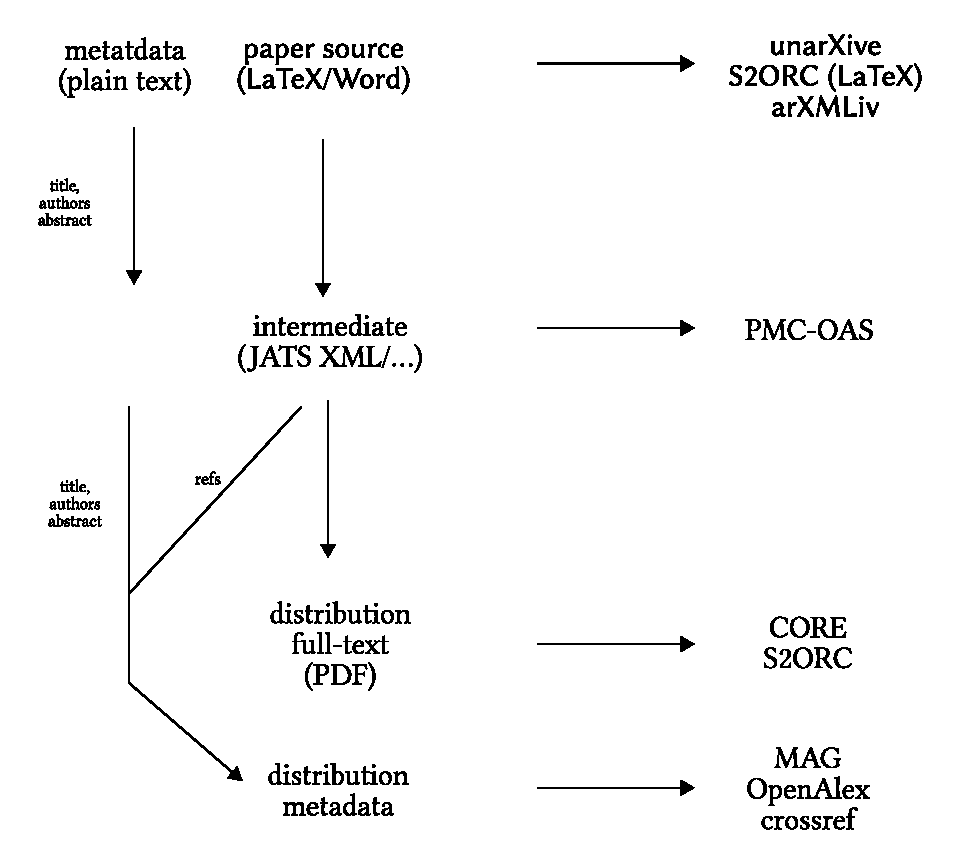
\includegraphics[width=0.7\linewidth]{figures/foundations/scholarly_data_lifecycle_dummy}
  \caption[Scholarly data origins]{Scholarly data origins (note: in text mention that for older publications it goes from some source to distribution on paper, and scholarly data then requires OCR on scanned documents)}
  \label{fig:foundations-datalifecycle}
\end{figure}


Figure~\ref{fig:foundations-datalifecycle} schematically shows the path of a publication from authorship to distribution, together with different stages from which scholarly data can emerge. It is essential to note that academic publications are, historically and at the time of writing still, primarily written by humans with human readership in mind. As such, publications are primarily a visual medium, optimized for parsing by human vision and intelligence. Scholarly data, however, is intended for automated processing and therefore benefits, for example, from strict syntactic rules and no reliance on assumed background knowledge. As a consequence, the creation of scholarly data requires bridging between the existing visual presentation and desired structural derivate.

Specifically, this means that information which is not made explicit in publications needs to be retroactively added. For example, if a piece of text \textit{``[1-3]''} in a publication is expressing a value rage, or a citation for references 1 to 3. Because it would be impractical to require researchers to produce a detailed set of annotations in addition to all their publications,\footnote{An exception to this is basic metadata such as title, authors, and abstract, which are commonly requested to be filled into a form in plain text during the submission process of a manuscript.} the retroactive adding of information needs to be done automatically, i.e. by means of information extraction. An shown in Figure~\ref{fig:foundations-datalifecycle}, the information extraction can happen at any given stage of publication. At each stage, the nature of the available data and information is different. Accordingly, there are different benefits and challenges. In the following we will discuss these different types of data, beginning with \LaTeX\ as it is the most relevant to the presented work.

\subsubsection{Data Formats}

\paragraph{\LaTeX}

% The STM Report
% SALT: Weaving the Claim Web

% - LaTeX; what is it, why is it not the end-all-be-all, and what endeavours have been there so far and are on the horizon of LaTeX development wrt. more structure and semantic information?
%   -> brief history, used primarily in STEM fields, Turing complete, document classes and packages provide semantic macros that translate in to visual representation but authors can always chose to directly describe visual presentation rather than semantic meaning, some endeavours to allow for more semantics (scholarly data specific and from accessibility POV)
% - What about other formats?
%   -> JATS is mighty, Word is XML, triple formats are used for metadata

Joanne Cohn sending around e-prints~\cite{Feder2021,Turner2012}

June 1991 meets Paul Ginsparg who then goes on to start arXiv~\cite{Ginsparg2011a,Ginsparg2011}

arXiv used 1998 for scholarly IE~\cite{Nanba1998}

Semantic annotation natively from \LaTeX\ in the works (w/ accessibility in mind)~\cite{Mittelbach2020}

metadata dump since 2020(?) available on Kaggle~\cite{arxiv_kaggle_dataset}

\paragraph{Word}

\paragraph{JATS XML}

\paragraph{PDF}

\paragraph{Triple Formats}
RDF, Turtle, JSON-LD, ... (relevant for metadata)

% document classes and packages provide semantic macros and translate them
% into visual output, but user can at any time also use visual primitives
% directly

\subsubsection{Types of Scholarly Data}
% What do I want to say and convey here?

% - what ``conceptual'' types of scholarly data are there?
%   -> metadata, document collections, linked document collections (combining former two b/c metadata usually also means citations)
% - what are current/established (``SOTA'') approaches/endeavors/projects
%   -> ORKG (very semantic but not scalable yet), arXMLiv (math focus), S2ORC (PDF source), OpenAlex (very large, ...)

\section{Data Mining \& Information Extraction}

% What do I want to say and convey here?
% - 

\subsection{Data Quality Metrics}

\subsection{Model Evaluation Metrics}
